\documentclass[12pt, letter]{article}

% Load packages
\usepackage[style = authoryear, autocite=inline, doi=false,isbn=false,url=false]{biblatex}
\usepackage[margin = 1 in]{geometry}
\usepackage[colorlinks, citecolor = red]{hyperref}
\usepackage{amsmath, amssymb} %essential
\usepackage[long, nodayofweek]{datetime}
\usepackage[]{booktabs}
\usepackage{graphicx}
\usepackage{setspace}
\usepackage{todonotes}
\usepackage[font=small,labelfont=bf]{caption}

% Define symbols
\DeclareRobustCommand{\bbone}{\text{\usefont{U}{bbold}{m}{n}1}}
\DeclareMathOperator{\EX}{\mathbb{E}} % expected value
\DeclareMathOperator{\V}{\mathbb{V}}
\DeclareMathOperator{\Prob}{\mathbb{P}}
\newcommand*{\trans}{^{\mathsf{T}}} %matrix transpose


\begin{document}

% Define Header
\author{Andrew C. Eggers\thanks{Nuffield College and Department of Politics and International Relations, University of Oxford, United Kingdom. \texttt{aeggers@nuffield.ox.ac.uk}}
\and
Tobias Nowacki\thanks{Department of Political Science, Stanford University, CA, United States. \texttt{tnowacki@stanford.edu}}}
\date{\today}
\title{Comparing strategic voting incentives in plurality and instant-runoff elections}

\maketitle

\onehalfspacing % set line space

\setcounter{section}{3}

\section{Data}


To assess the prevalence and distribution of strategic incentives under plurality and IRV empirically, we rely on the Comparative Study of Electoral Systems (CSES) data for a realistic set of preferences and beliefs. The dataset covers 160 surveys from xx different countries, administered shortly before or after an election.\footnote{Two additional cases in the survey, Belarus (20xx) and Lithuania (20xx), are dropped because no respondent specified full preferences over more than two parties.} We focus on the three largest parties (evaluated how?) and label them $A, B, C$ in descending size, respectively. From each survey, we take the party like/dislike scores to approximate voters' ordinal utilities and construct their preference ranking. Let $\bf \tilde{v}$ be the vector of ballot proportions if everyone in the survey voted sincerely. Then, we assume that respondents' beliefs about the next election can be captured with a $\text{Dir}(s \times \bf \tilde{v})$ distribution. Using this set up, we can calculate the strategic incentives under either electoral system as laid out in Section 2.

We should begin with the caveat that a theory that incorporates all relevant parameters (utilities, beliefs, information, etc.) and their respective interactions would be too demanding. Instead, we intend to give our readers a broad sketch of the main theoretical implications; the subsequent presentation of results will address these and explain additional patterns in the data.

\subsection{Summary statistics}

\begin{figure}[!htb]
	\centering
	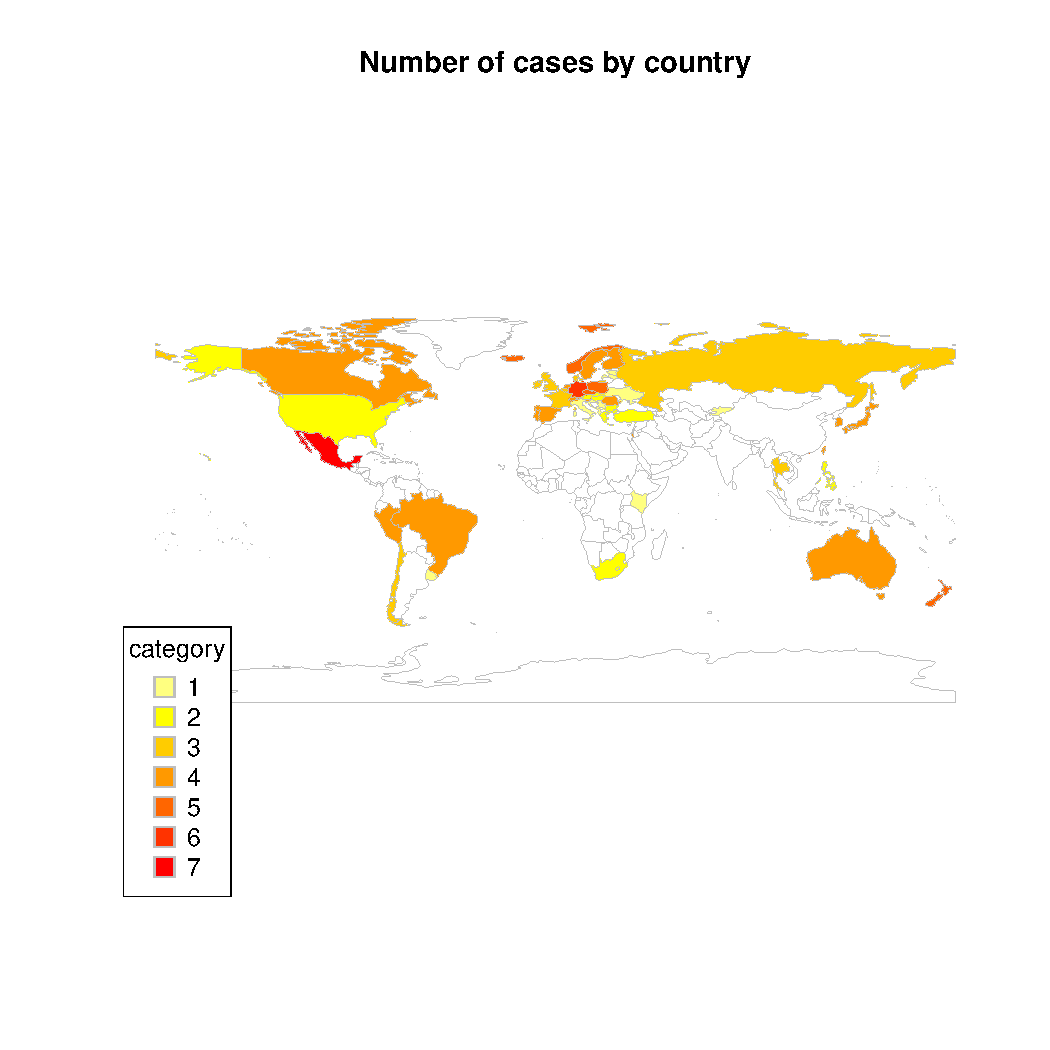
\includegraphics[width = .5 \textwidth]{../output/figures/case_map.pdf}
	\caption{Cases in CSES data, by country}
	\label{fig:case_map}
\end{figure}

The mean number of respondents in each case is 1384 (with a standard deviation of 539). The 160 different surveys come from xx different countries from the time between 1996 and 2016. Figure~\ref{fig:map} maps the number of surveys in each country. (Do we need to say any more? Perhaps something about mean / sd of preference intensity and $\tau$?)

\subsection{Distribution of preferences} 

How different are the CSES cases from one another? Aside from the intensity of preferences, we can describe each case with the vector $\bf \tilde{v}$, where the three-item vector $(v_1 + v_2, v_3 + v_4, v_5 + v_6)$ describes the distribution of first preferences, and the three-item vector $(m_{AB} = \frac{v_1}{v_1 + v_2}, m_{BA} = \frac{v_3}{v_3 + v_4}, m_{CB} = \frac{v_6}{v_5 + v_6})$ describes the distribution of second preferences. 

To link these two distributions together and classify cases more completely, we offer the following approach. Without loss of generality, let the candidate (party) $X$ whose first-preference voters have the most equally split second preferences, and the other two parties $Y$ and $Z$. If both $m_{YZ}$, $m_{ZY} > 0.6$, then classify this case as \emph{single-peaked} and denote it $X+$.\footnote{$X$ is the attractor: both remaining parties have a majority of their second preferences tilted towards $X$.} Conversely, if both $m_{YZ}, m{ZY} < 0.4$, then classify this case as \emph{divided majority} and denote it $X-$.\footnote{Here, $X$ is the repeller: both remaining parties have a majority of their second preferences tilted towards each other and away from $X$.} If $m_{YZ}, m_{ZY} \in [0.4, 0.6]$, then classify this case as \emph{neutral} and denote it $N(X)$. If neither of these conditions hold (because of unusual second preferences), classify it as \emph{other} and denote it $O$. This completes a mutually exclusive and exhaustive set of classes determined by $\bf \tilde{v}$.

\begin{table}[tb]
	\caption{Distribution of preference profiles in CSES data}
	\label{tab:csesprefs}
	\centering

	\begin{tabular}{lccc}
	\hline

	\toprule
	\textbf{} & \textbf{A} & \textbf{B} & \textbf{C} \\
	\cmidrule{2-4}
	Single-peaked (+) & 18 & 23 & 9  \\
	Divided majority (-) & 28 & 20 & 20  \\
	Neutral () & 5 & 7 & 3  \\
	Other () & & 27 &  \\
	\bottomrule
	\end{tabular}
\end{table}

Table~\ref{tab:csesprefs} summarises the distribution of preference classes across the CSES cases. A plurality of cases belong to the divided majority classes; however, there is also a large number of single-peaked cases, whereas neutral and others tend to be rarer. (Figure~\ref{fig:cses_fp} plots the distribution of first preferences conditional on the classes.)

\begin{figure}[!htb]
	\centering
	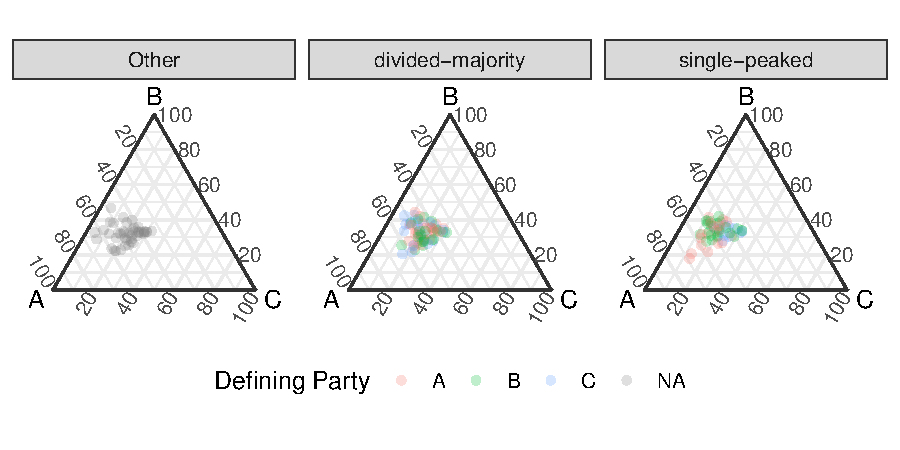
\includegraphics[width = 0.6 \textwidth]{../output/figures/cses_fp.pdf}
	\caption{Distribution of first preferences in CSES cases, by class}
	\label{fig:cses_fp}
\end{figure}

\section{Results: Baseline Case}

Section 2 describes our analytical approach, which we apply to the CSES data described in Section 4. For each case in the CSES, we obtain a matrix $\bf X$, where the rows correspond to respondents, and each row $x_i\trans = [\tau_{Ii}, \tau_{Pi}]$.\footnote{Shorthand notation: $\tau_{I}$ is the strategic incentive under \textbf{I}RV, and $\tau_{P}$ is the strategic incentive under \textbf{P}lurality.} In this section, we present our main results for the baseline case, where we assume that every voter is Level-1 strategic; that is, they expect everyone else to vote sincerely. We describe the distribution of $\tau$ under either electoral system, focussing on the prevalence and magnitude of positive strategic incentives. Our main finding is that, for our input of representative preference data from 160 elections, Level-1 voters are more likely to have positive strategic incentives under IRV than under Plurality ($
\Prob(\tau_{I} > 0) > \Prob(\tau_{P} > 0)$); however, conditional on having a positive incentive, its magnitude will be larger under Plurality ($\EX[\tau_{P} | \tau_{P} > 0] > \EX[\tau_{I} | \tau_{I} > 0]$). These findings are consistent with our theoretical expectations.\footnote{We emphasise that these are probabilistic statements -- our findings hold in expectation, across the sample of elections from all over the world. As the data for individual cases shows, there are instances where, given the country's preference profile, Plurality yields a greater prevalence of strategic voting and/or smaller expected magnitudes.} To compare the performance of the two systems more broadly, we also check the probability of electing the Condorcet winner conditional on the share of Level-1 strategic versus sincere voters. We find that, ...

\subsection{Prevalence of Strategic Incentives}

First, we show the raw proportion of voters with $\tau > 0$ in each case (which we call prevalence). If $P_j$ is the distribution of preferences in case $j$, then this is simply defined as:

\begin{equation}
\Prob(\tau_{k \, i} > 0 | P_j)	
\end{equation}

Figure \ref{fig:sv_prop} plots the prevalence of strategic incentives of each case under the two electoral systems at various levels of . The 45-degree line indicates cases where the prevalence is equal under either electoral system; cases above see more prevalent strategic incentives under IRV, and cases below see more prevalent strategic incentives under Plurality.

\begin{figure}[!htb]
	\centering
	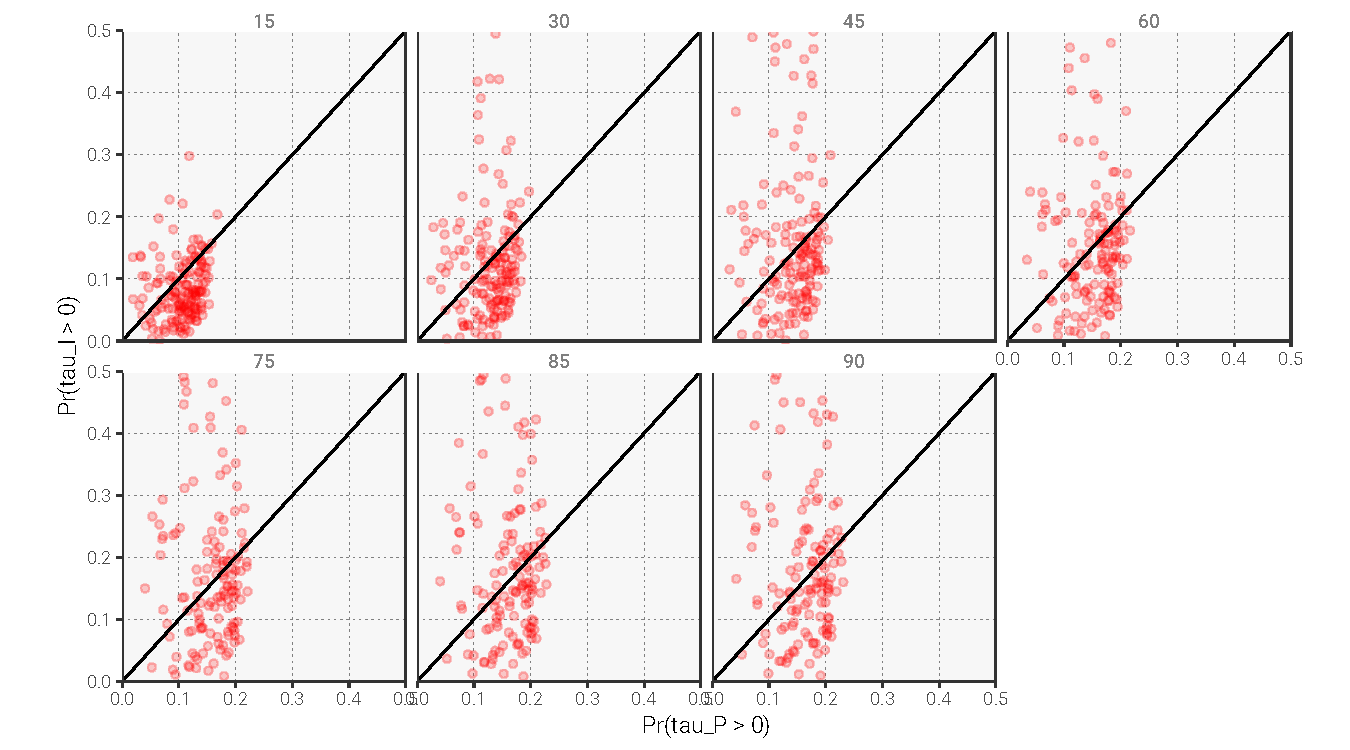
\includegraphics[width = 0.8 \textwidth]{../output/figures/cses_prop.pdf}
	\caption{Prevalence of strategic incentives.}
	\label{fig:sv_prop}
\end{figure}

At low levels of information (that is, high uncertainty in beliefs about $\bf v$), strategic incentives are, overall, more prevalent under Plurality. This is in line with our theoretical expectations: even with high uncertainty, supporters of a small third party will expect a small probability of their candidate being tied with the expected frontrunner; in relative terms, the probability of the expected top two candidates tying is still higher, and thus there is still an incentive for supporters of the third party to vote strategically. (Note that the proportion under plurality is capped at around 0.2, and stays at that level regardless of $s$).

Under IRV, the high uncertainty means that many different pivotal events are likely, many of which suggest conflicting optimal votes. As a result, voters are best off staying with their sincere preference ordering. 

As uncertainty about the expected outcome decreases (and $s$ increases), the prevalence of strategic incentives increases for a number of cases under IRV, but not under Plurality. These are cases where the expected outcome (i.e. the centre of the beliefs) is close to a pivotal event that induces a particular strategic incentive, and somewhat farther to other pivotal events that induce conflicting vote choices. With shrinking uncertainty, the probability of the former increases and the probability of the latter decreases; as a result, $\tau$ increases (and, it seems in many cases, crosses $\tau = 0$). Because of the paucity of pivotal events under Plurality, no similar dynamic occurs here.\footnote{Actually, looking at the series of plots from $s = 15$ to $s = 90$, there is \emph{some} expansion of the threshold from about 0.15 to about 0.20.}

Another noteworthy result is that this increase under IRV only holds true for a subset of cases (primarily the ones that we classify as $B+$ and $C-$). This speaks to the importance of the preference input; it is possible to construct scenarios that lead to drastically different comparisons. By taking a wide and representative sample from elections across the entire world we attempt to provide a sketch of strategic incentives under likely, real-world preference distributions.

\subsection{Magnitude of Strategic Incentives}

Next, we want to examine the magnitude of these incentives: beyond knowing \emph{whether} voters can improve their expected utility by voting strategically, we also want to know by how much they can do so. To present an aggregate result that is representative of the total electorate across our cases, we weight each observation based on sample size and country's electorate population:

\begin{equation*}
	\tilde{w}_{ijk} = w_{ijk} \frac{N_k}{ n_{jk} m_{k} } 
\end{equation*}

where $w_{ijk}$ is the original weight from the CSES data, $N_k$ is the size of the electorate in country $k$, $n_{jk}$ is the sample size of the survey $j$in country $k$, and $m_k$ is the number of surveys in country $k$. After assigning weights, we then run a simple weighted regression model on respondents' strategic incentives under both $\tau_I$ and $\tau_P$ when $s = 85$:

\begin{equation}
	D_i = \beta_0 + \beta_1 IRV_i + \eta_i
\end{equation}

where $D_i$ is a binary variable that is 1 if $\varepsilon > 0$ and 0 otherwise. The coefficient $\hat{\beta_1}$ is then the difference between the proportion of weighted voters with $\tau_{I} > \varepsilon$ and $\tau_{P} > \varepsilon$. Put differently, we estimate the quantity

\begin{equation*}
	\int_\varepsilon^\infty F(\tau_I) \ d\tau_I - \int_\varepsilon^\infty G(\tau_P) \ d\tau_P
\end{equation*}

for a range of $\varepsilon$. We run the above regression model for a range of values of $\varepsilon$ and report the results graphically, with standard errors clustered by respondent, in Figure~\ref{fig:sv_epsilon}

\begin{figure}[!htb]
	\centering
	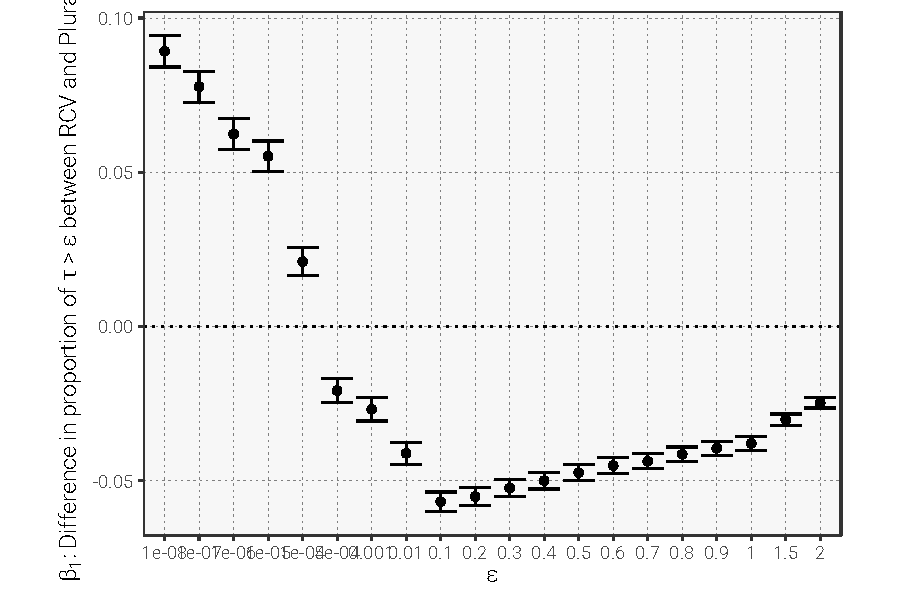
\includegraphics[width = 0.8 \textwidth]{../output/figures/epsilon_factor_scale.pdf}
	\caption{Magnitude of strategic incentives.}
	\label{fig:sv_epsilon}
\end{figure}

As discussed in the previous subsection, $\Prob(\tau_I > 0) > \Prob(\tau_P > 0)$. However, as $\varepsilon$ increases, that difference shrinks and becomes negative at $\varepsilon \sim 0.001$. This indicates that a large proportion of the positive strategic incentives under IRV have a very small magnitude: the expected utility benefit over a sincere vote is relatively minor. Consequently, conditional on voters with $\tau_P > 0$, the expected magnitude of that strategic incentive will be larger. Note that the difference creeps back towards equality at very high levels of $\varepsilon$, which indicates that extremely high values of $\tau$ are, once again, more equally distributed between the two electoral systems.\footnote{The upshot is that under IRV, most magnitudes are very small, but there seem to be a few extreme outliers with very large $\tau$.}

Once again, we derive the intuition for this result from our theoretical framework: under IRV, the number and conflicting nature of pivotal events yields more difficult decisions, whereas under Plurality, switching from the expected third place bears a clear benefit that is only contradicted by the unlikely case of one's first preference suddenly being competitive, after all.

What this means in practice is that, if we think of $\epsilon$ as the cost of having to forgo one's sincere ballot (e.g, the opportunity cost of the warm glow of sincerity), then, unless this cost is very small, the incentive to vote strategically under IRV all but disappears in most cases. We may speculate that this is one reason why IRV is frequently characterised as 'strategy-proof', but evaluating such a hypothesis remains the purview of future research.

\subsection{System-Level Performance}

Next, we show results for a system-wide comparison: how likely is it that the electoral system returns the Condorcet winner, given the set of CSES preferences and a proportion $\lambda$ that is Level-1 strategic?

For each CSES case, we ran the following procedure over 1000 iterations for each value of $\lambda$: first, we randomly sampled 300 respondents from the case survey. We then randomly assigned the proportion $\lambda$ to be level-1 strategic, and the remaining to be sincere voters. We aggregated the sample's hypothetical ballots, given assignment, and checked whether the Condorcet winner would be elected or not. The obtained proportion of the 1000 iterations where the Condorcet winner \emph{is} elected serves as our probability estimate conditional on the electoral system and the value of $\lambda$.

\begin{figure}[!htb]
	\centering
	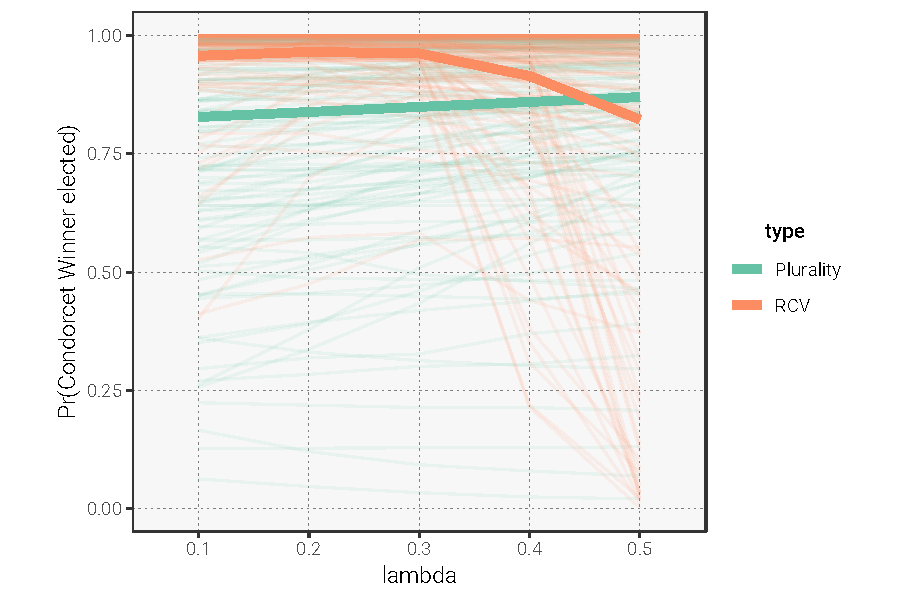
\includegraphics[width = 0.8 \textwidth]{../output/figures/condorcet_probs.pdf}
	\caption{Probability of electing the Condorcet Winner, given proportion of level-1 strategic voters ($\lambda$). Thick lines indicate (unweighted) aggregate results across all cases.}
	\label{fig:sv_condorcet}
\end{figure}

Figure~\ref{fig:sv_condorcet} summarises the results of the above procedure for values $\lambda \in [0.1, 0.2, 0.3, 0.4, 0.5]$. For low and intermediate values of $\lambda$, IRV elects the Condorcet winner in more than 90\% of simulations (on average, though the specifics depend, as always, on the preference input and the case). The probability exhibits much more variance across cases under Plurality, and is, on average, lower. At high values of $\lambda$, the probability under IRV begins to decrease and falls below that of Plurality, driven by a few extreme cases. This region of $\lambda$, however, is highly unlikely to occur in reality: it would require that at least half of all voters vote strategically.\footnote{They may be strategically minded, but where $\tau_{Ii} < 0$, they will still submit a sincere ballot.} (cf., for example, Abramson et al. 2010, for estimates of the prevalence of strategic \emph{voting}). 
Overall, we conclude that, on aggregate, for a realistic set of preferences, and reasonable proportions of strategic voters, IRV performs better in electing the Condorcet Winner than Plurality.

\section{Results: Interdependence}

(\emph{We should probably introduce the level-1, level-2, etc. concepts with formal language somewhere.})

So far, we considered the strategic incentives of each voter in isolation, and only distinguished between level-0 (sincere) and, at best, level-1 voters. Yet, strategic voting can also have complementary and substitution effects. 

\subsection{Intuition}

Consider the following scenario under Plurality. There is a mass of voters whose first preference is for $C$ (whom they expect to come third). There is an incentive to abandon $C$ and vote for $A$ or $B$ -- either of the two frontrunners -- instead, thus increasing one's probability of casting a pivotal ballot. Yet, the greater the proportion of sincere $C$ voters does so, the stronger will my incentive be to follow suit, because $C$'s expected vote share will decrease even further. Thus, under Plurality, strategic incentives are complementary. 

Under IRV, the interdependence is not as clear-cut. There are different types of strategic votes (cf. Section 3), which depend on different pivotal events. Some of them mechanically induce a complementarity effect whilst others (e.g,. strong pushover) induce a substitution effect. Strong pushover suggests that voters, e.g., ($ABC$) should put their third preference ($C$) first in order to advance it to the run-off, where it $A$ can beat $C$ but not $B$. However, if every voter with a sincere preference for $A$ did so, then, eventually, $C$
would also beat $A$ in the run-off as a result of the additional strategic votes. Hence, in this case, only a fraction of $ABC$ voters should embark on the strong pushover strategy. (This is a classic co-ordination dilemma.)

The implications of the different strategic nature of the two electoral systems, as illustrated by the above example, are that we expect IRV to have much less stable strategic incentives: my optimal ballot will vary much more depending on how strategic the other voters are.

\subsection{Results}

To check this intuition, we proceeded as follows: We assume that there is a proportion $\lambda$ of level-1 strategic voters, and $(1 - \lambda)$ sincere voters. The assignment of strategicness is uniform across all types of voters, such that the resulting expected outcome for a level-2 strategic voter (who has knowledge of $\lambda$ and anticipates this proportion voting strategically) is:

\begin{equation*}
	\tilde{\bf v}_{L2, \lambda} = \lambda {\bf v}_{L1} + (1 - \lambda) {\bf v}_{L0} 
\end{equation*}

We then compute the strategic incentive for a level-2 strategic voter by modelling their beliefs based on $f(\tilde{\bf v}_{L2, \lambda})$ instead of $f(\tilde{\bf v}_{L0}$.

\begin{figure}[!htb]
	\centering
	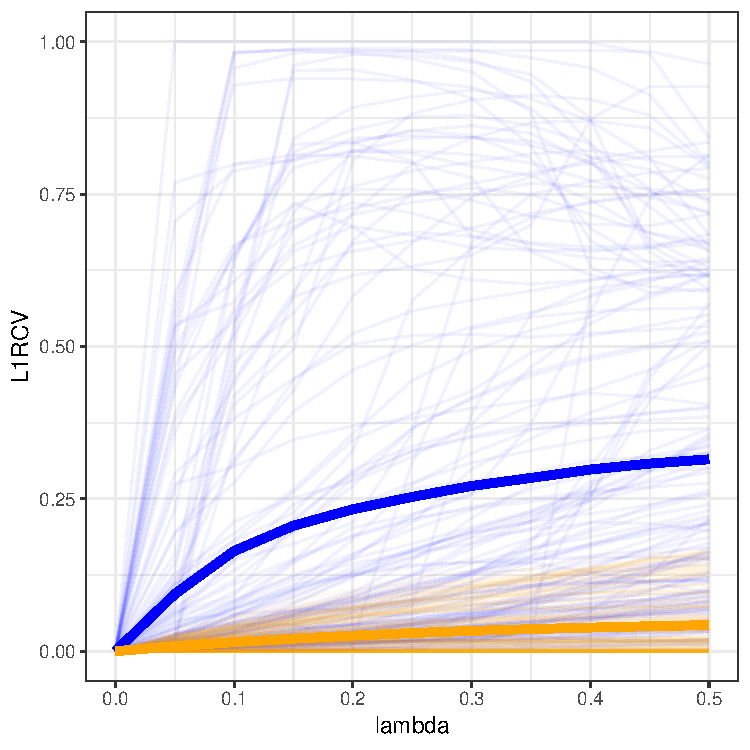
\includegraphics[width = 0.6 \textwidth]{../output/figures/cses_l1.pdf}
	\caption{Proportion of voters with optimal vote that differs between level-1 and level-2($\lambda$) strategicness.}
	\label{fig:sv_l1}
\end{figure}

Figure~\ref{fig:sv_l1} plots the proportion of respondents whose optimal vote differs when they are a level-2 strategic voter versus when they are a level-1 strategic voter. In line with the intuition, we see that as $\lambda$ increases, an increasing proportion of voters sees their optimal vote change as they move from level-1 to level-2 under IRV, but not under Plurality. (Note that the figure does not distinguish between voters who switch back to sincereity, and voters who switch to other ballots.) Under IRV, the average proportion across all cases rises to as much as 0.3 (when $\lambda = 0.5$), whereas under Plurality, it stays below 0.05.

\begin{figure}[!htb]
	\centering
	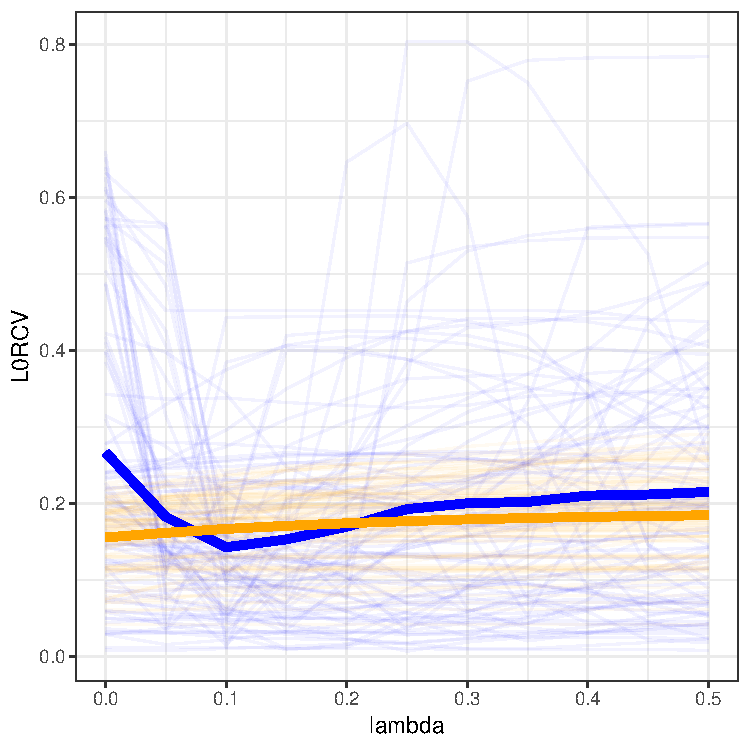
\includegraphics[width = 0.6 \textwidth]{../output/figures/cses_l0.pdf}
	\caption{Proportion of voters with optimal vote that differs between level-0 (sincerity) and level-2($\lambda$) strategicness.}
	\label{fig:sv_l0}
\end{figure}

Figure~\ref{fig:sv_l0} plots the proportion of respondents whose optimal vote differs when they are level-2 strategic versus their sincere vote. Here, we see the two cross-case averages roughly match each other at almost all levels of $\lambda$, although the variance of individual cases is much higher under IRV. However, there are two different mechanisms at work here: in Plurality, there is not much change between level-1 and level-2 voters, such that the proportion in Figure~\ref{fig:sv_l0} stays constant (those whose optimal L1 vote is non-sincere will also have a non-sincere L2 vote). Under IRV, in contrast, there are some voters who, by way of moving from L1 to L2, switch back to sincerity, and others who, at the same time move from sincerity in L1 to non-sincere optimal votes under L2. Thus, we see a lot change moving from level 1 to level 2, but in the aggregate it does not affect the balance between level 0 (sincerity) and level 2. (\emph{Can we provide more examples of this?})

Overall, the results confirm our theoretical intuition: interdependence of strategic incentives is much more sensitive under IRV. This adds an additional layer of complexity to voters acting strategically in this electoral system: not only do positive strategic incentives under IRV require high information precision, but voters must also have accurate beliefs about other voters' strategicness. This contributes to the likely scarcity of realised strategic voting under IRV (though, again, we do not intend to test this implication in this paper).

\section{Conclusion}



\end{document}